\documentclass[9pt]{beamer}
\usetheme{boxes}
\usetheme{Boadilla}
\usecolortheme{beaver}
%\usecolortheme{sidebartab}
% \usefonttheme{structurebold}
\usefonttheme{serif}

%gets rid of bottom navigation bars
\setbeamertemplate{footline}[page number]{}

%gets rid of navigation symbols
\setbeamertemplate{navigation symbols}{}


% \usepackage{helvet}
\usepackage{amsmath, amssymb}
\usepackage{color}
%\usepackage{asymptote}
\usepackage{mathrsfs}
\usepackage{dsfont}
\usepackage{url}
\usepackage{cancel}
\usepackage{tikz}
\usetikzlibrary{fit,positioning}
\usetikzlibrary{shapes,matrix,decorations.markings,arrows}
\usetikzlibrary{graphs}
\usepackage{bbm}
\def\ind{\mathbbm{1}} %Indicator function


%
\definecolor{darkblue}{rgb}{0.0, 0.0, 0.55}
\setbeamercolor{title}{fg=darkblue}
\setbeamercolor{frametitle}{fg=darkblue}
\newcommand{\myitem}{\item[$\bullet$]}
\definecolor{darkgreen}{rgb}{0, 0.55, 0}


\newcommand{\LABEQ}[1]{\label{eq:#1}}%\mathtt{[eq:#1]}\qquad
\newcommand{\LABALG}[1]{\label{alg:#1}}%\mathtt{[lab:#1]}\qquad
\newcommand{\LABTAB}[1]{\label{tab:#1}}%{\tt [tab:$\text{$#1$}$]}}
\newcommand{\LABFIG}[1]{\label{fig:#1}}%{\tt [fig:$\text{$#1$}$]}}
\newcommand{\LABTHM}[1]{\label{thm:#1}}%{\tt [thm:#1]}}
\newcommand{\LABPRP}[1]{\label{prp:#1}}%{\tt [prp:#1]}}
\newcommand{\LABLEM}[1]{\label{lem:#1}}%{\tt [lem:#1]}}
\newcommand{\LABCOR}[1]{\label{cor:#1}}%{\tt [cor:#1]}}
\newcommand{\LABDFN}[1]{\label{dfn:#1}}%{\tt [dfn:#1]}}
\newcommand{\LABFNT}[1]{\label{fnt:#1}}%{\tt [fnt:#1]}}
\newcommand{\EQ}[1]{\eqref{eq:#1}}%$^{\text{\tt [#1]}}$} %used to be  %{(\ref{eq:#1})}
\newcommand{\ALG}[1]{~\ref{alg:#1}}
\newcommand{\TAB}[1]{~\ref{tab:#1}}%$^{\text{\tt [#1]}}$}
\newcommand{\FIG}[1]{\ref{fig:#1}} %$^{\text{\tt [#1]}}$}
\newcommand{\THM}[1]{~\ref{thm:#1}}%$^{\text{\tt [#1]}}$}
\newcommand{\COR}[1]{~\ref{cor:#1}}%$^{\text{\tt [#1]}}$}
\newcommand{\PRP}[1]{~\ref{prp:#1}}%$^{\text{\tt [#1]}}$}
\newcommand{\LEM}[1]{~\ref{lem:#1}}%$^{\text{\tt [#1]}}$}
\newcommand{\DFN}[1]{~\ref{dfn:#1}}%$^{\text{\tt [#1]}}$}
\newcommand{\FNT}[1]{~\ref{fnt:#1}}%$^{\text{\tt [#1]}}$}
\newcommand{\PAGEEQ}[1]{~\pageref{eq:#1}}
\newcommand{\PAGETAB}[1]{~\pageref{tab:#1}}
\newcommand{\PAGEFIG}[1]{~\pageref{fig:#1}}
\newcommand{\LABCHAP}[1]{\label{chap:#1}}%{\tt [chap:#1]}}
\newcommand{\LABSEC}[1]{\label{sec:#1}}%{\tt [sec:#1]}}
\newcommand{\LABSSEC}[1]{\label{ssec:#1}}%{\tt [ssec:#1]}}
\newcommand{\LABSSSEC}[1]{\label{sssec:#1}}%{\tt [sssec:#1]}}
\newcommand{\CHAP}[1]{~\ref{chap:#1}}%$^{\text{\tt [c:#1]}}$}
\newcommand{\SEC}[1]{~\ref{sec:#1}}%$^{\text{\tt [s:#1]}}$}
\newcommand{\SSEC}[1]{~\ref{ssec:#1}}%$^{\text{\tt [ss:#1]}}$}
\newcommand{\SSSEC}[1]{~\ref{sssec:#1}}%$^{\text{\tt [sss:#1]}}$}


\def\len{L}
\newcommand{\ve}[1]{\boldsymbol{#1}}
\newcommand{\set}[1]{\mathcal{#1}}

\def\x{m}
\newcommand{\st}[1]{{g}_{#1}}		%state
\newcommand{\stp}[1]{{g}'_{#1}}		%state
\newcommand{\str}[2]{{g}_{#2,(#1)}}	
\newcommand{\St}[1]{{G}_{#1}}		%state

\newcommand{\p}[1]{p_{_{#1}}} %pdf or pmf
\newcommand{\pmd}[1]{\tilde{p}_{_{#1}}} %pdf or pmf
\newcommand{\q}[1]{q_{_{#1}}} %pdf or pmf
\newcommand{\Iset}[1]{\mathtt{#1}} %Index set
\def\d{\text{d}}	%Differential (for integrals)
\newcommand{\va}[3]{#1^{(#2)}_{#3}}

\usepackage{pst-sigsys,pst-plot,pstricks-add}
%\usepackage{auto-pst-pdf}
\usepackage{pst-pdf}
\usepackage{pgfplots}
\usetikzlibrary{external} %pdflatex -shell-escape mydocument.tex
%\tikzset{external/force remake}
\tikzexternalize[prefix=tikzgraphics/]

\definecolor{mycolor1}{rgb}{0.6000,1,0.00000}
\definecolor{mycolor2}{rgb}{0.00000,0.75,0.75000}
\definecolor{mycolor3}{rgb}{0.95,0.95,0.95000}

\newcommand{\mc}[1]{\mathcal{#1}}
\def\sX{\mc{X}}

\newcommand\Def[1]{{\textbf{Definition:}\\\emph{#1}\\\begin{center} ------------------------ \end{center}}}
\newcommand\Prop[1]{{\textbf{\textcolor{red}{Property:}}\\\emph{#1}\\\begin{center} \textcolor{red}{------------------------} \end{center}}}

\newcommand{\noteB}[1]{\textbf{\textcolor{darkblue}{#1}}}

\newcommand{\noteR}[1]{\textbf{\textcolor{darkred}{#1}}}

\newcommand{\noteG}[1]{\textbf{\textcolor{darkgreen}{#1}}}

\newcommand{\snoteB}[1]{{\textcolor{darkblue}{#1}}}

\newcommand{\snoteR}[1]{{\textcolor{darkred}{#1}}}

\newcommand{\snoteG}[1]{{\textcolor{darkgreen}{#1}}}


\newcommand{\fs}[2]{#2}

\title[]{A short introduction to Turbo Coding}
\author[\textcolor{white}{Advanced Digital Communications}]{Introduction to Graphical Models and Inference for Communications\\\vspace*{3mm}{\small \textcolor{black}{UC3M}}
}
%\date[08/02/2016]{{08/02/2016}}
\institute{\textcolor{white}{}}

% \pgfdeclareimage[height=0.5cm]{ITW}{pics/Logo.png}
%  \logo{\pgfuseimage{ITW}}

\AtBeginSection[]
{
  \begin{frame}<beamer>{Index}
    \tableofcontents[currentsection,currentsubsection]
  \end{frame}
}

\begin{document}

\frame{
\titlepage
\thispagestyle{empty}
\begin{center}
\includegraphics[scale=0.05]{Figuras/uc3m-logo.pdf}
\end{center}
}

\frame{
\frametitle{Today}

\begin{itemize}
\item Turbo Codes
\item Encoder structure
\item Interleaver
\item Decoding
\item Introduction to Lab. project 2
\end{itemize}

}

\frame{
\frametitle{Turbo Codes}

\begin{itemize}
\item  High-performance forward error correction (FEC) codes developed around 1990-91 (but first published in 1993).
\end{itemize}

\begin{itemize}
\item  First practical known codes to closely approach the channel capacity.
\end{itemize}

\begin{itemize}
\item   3G/4G mobile communications (e.g. in UMTS and LTE) and in (deep space) satellite communications.
\end{itemize}
}

\frame{
\frametitle{Econder structure}

\begin{itemize}
\item   Two convolutional codes in parallel with some kind of interleaving in between.
\end{itemize}

\begin{figure}[h!]
\begin{center}
%\tikzset{external/remake next}
% This file was created by matlab2tikz.
% Minimal pgfplots version: 1.3
%
%The latest updates can be retrieved from
%  http://www.mathworks.com/matlabcentral/fileexchange/22022-matlab2tikz
%where you can also make suggestions and rate matlab2tikz.
%


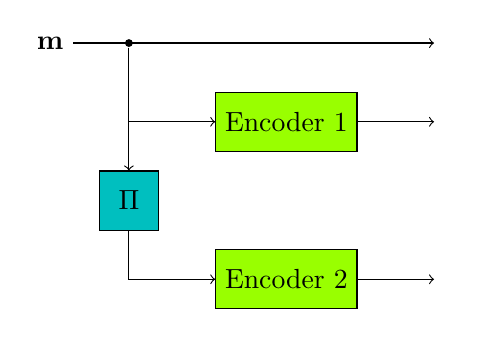
\begin{tikzpicture}[%
%    node distance = 2 cm,auto,>=latex',
    block3/.style  = {draw, rectangle, minimum width = 0.75cm, minimum height = 0.75cm,fill=mycolor1},
        block4/.style  = {draw, rectangle, minimum width = 0.75cm, minimum height = 0.75cm,fill=mycolor2},
    sum/.style    = {draw, circle, minimum size=.5cm, node distance=1.25cm},
    input/.style  = {coordinate},
    output/.style = {coordinate},
    dot/.style    = {anchor=base,fill,circle,inner sep=1pt}]

  \draw (-2,2) node [] (input) {$\mathbf{m}$}; 
  \draw (1,1) node[block3]  (En1) {Encoder 1};  
  \draw (-1,0) node[block4]  (Int) {$\Pi$};  
   \draw (1,-1) node[block3]  (En2) {Encoder 2};  
   \draw (3,2) node [] (out1) {}; 
   \draw [->] (input) -- (out1);
   \draw (-1,2) node[dot] (p1) {};
   \draw [->] (p1) |- (En1);
   \draw [->] (p1) -- (Int);
   \draw [->] (Int) |- (En2);
    \draw (3,1) node [] (out2) {}; 
    \draw (3,-1) node [] (out3) {}; 
  \draw [->] (En1) -- (out2);
  \draw [->] (En2) -- (out3);
  
   
\end{tikzpicture}% 
\end{center}
\caption{Turbo code encoder structure}\label{fig0}
\end{figure}

\begin{itemize}
\item   The frames can be terminated - i.e. the encoders are
forced to a known state after the information block. The termination tail is then appended to
the encoded information and used in the decoder. 
\end{itemize}

}

\frame{
\frametitle{3GPP RSC code}

\begin{figure}[h!]
\begin{center}
%\tikzset{external/remake next}
\input{tikzfiles/Fig1.tex} 
\end{center}
\caption{Rate-1/2 RSC Convolutional Code}\label{fig1}
\end{figure}

}

\frame{
\frametitle{3GPP RSC Turbo code}

\begin{figure}[h!]
\begin{center}
%\tikzset{external/remake next}
% This file was created by matlab2tikz.
% Minimal pgfplots version: 1.3
%
%The latest updates can be retrieved from
%  http://www.mathworks.com/matlabcentral/fileexchange/22022-matlab2tikz
%where you can also make suggestions and rate matlab2tikz.
%

\definecolor{mycolor1}{rgb}{0.00000,0.5,0.00000}

\begin{tikzpicture}[%
\tikzstyle{factor}=[rectangle,minimum size = 5mm, thick, draw =black,fill=black]
\tikzstyle{var}=[circle,minimum size = 5mm, thick, draw =black,fill=black]
\tikzstyle{second}=[circle, minimum size = 10mm, thick]
\tikzstyle{box}=[rectangle, draw=black!100]
\tikzstyle{connect}=[-latex, thick]

	
	\node[factor] (tphi0) at (0,0) [label=below:{$\ind[\st{0}=\st{}^*]$}]{};
	\node[var] (phi0) at (2,0) [label=above:{$\st{0}$}]{};
	\node[factor] (tphi1) at (4,0) [label=below:{$t_0$}]{};
	\node[var] (s0) at (4,2) [label=left:{$S_0$}]{};
	\node[factor] (fs0) at (4,4) [label=above:{$\p{S_0}$}]{};
	
	\node[var] (phi1) at (6,0) [label=above:{$\st{1}$}]{};
	\node[factor] (tphi2) at (8,0) [label=below:{$t_1$}]{};
	\node[var] (s1) at (8,2) [label=left:{$S_1$}]{};
	\node[factor] (fs1) at (8,4) [label=above:{$\p{S_1}$}]{};	

	
	\node[var] (phi2) at (10,0) [label=above:{$\st{2}$}]{};
	\node[factor] (tphi3) at (12,0) [label=below:{$t_2$}]{};
		\node[var] (s2) at (12,2) [label=left:{$S_2$}]{};
	\node[factor] (fs2) at (12,4) [label=above:{$\p{S_2}$}]{};		
	
	\node[var] (phi3) at (14,0) [label=above:{$\st{3}$}]{};
	\node[factor] (tphi4) at (16,0) [label=below:{$t_3$}]{};
	\node[var] (s3) at (16,2) [label=left:{$S_3$}]{};	
	\node[factor] (fs3) at (16,4) [label=above:{$\p{S_3}$}]{};
	
	\node[var] (phi4) at (18,0) [label=above:{$\st{4}$}]{};
	\node[factor] (tphi5) at (20,0) [label=below:{$t_4$}]{};
	\node[var] (s4) at (20,2) [label=left:{$S_4$}]{};	
	\node[factor] (fs4) at (20,4) [label=above:{$\p{S_4}$}]{};	
	
	\node[factor] (fs5) at (24,4) [label=above:{$\p{S_5}$}]{};	
	\node[var] (s5) at (24,2) [label=left:{$S_5$}]{};	
	\node[var] (phi5) at (22,0) [label=above:{$\st{5}$}]{};
	\node[factor] (tphi6) at (24,0) [label=below:{$t_5$}]{};	
	
	\node[factor] (fs6) at (28,4) [label=above:{$\p{S_6}$}]{};	
	\node[var] (s6) at (28,2) [label=left:{$S_5$}]{};	
	\node[var] (phi6) at (26,0) [label=above:{$\st{6}$}]{};
	\node[factor] (tphi7) at (28,0) [label=below:{$t_6$}]{};
	\node[var] (phi7) at (30,0) [label=above:{$\st{7}$}]{};
	\node[factor] (tphi8) at (32,0) [label=below:{$\ind[\st{7}=\st{}^*]$}]{};
	
	\path
		(tphi0) edge [] (tphi8)
		(fs0) edge [] (tphi1)
		(fs1) edge [] (tphi2)
		(fs2) edge [] (tphi3)
		(fs3) edge [] (tphi4)
		(fs4) edge [] (tphi5)
		(fs5) edge [] (tphi6)	
		(fs6) edge [] (tphi7);	
				
		
	
\end{tikzpicture}
   
 
\end{center}
\end{figure}

}

\frame{
\frametitle{Interleaver}

\begin{itemize}
\item Let $\len$ denote the length of the encoded sequence (we have to add the termination bits).
\end{itemize}

\begin{itemize}
\item The interleaver design is a key factor which determines the good performance of a turbo code.
\end{itemize}

\begin{itemize}
\item The input sequence to each of the two component RSC codes look ``almost'' independent.
\end{itemize}


\begin{itemize}
\item We need $\len\rightarrow\infty$ to approximate channel capacity.
\end{itemize}

}

\frame{
\frametitle{“Row-Column” interleaver}
\begin{itemize}
\item Simplest interleaver. Data is written row-wise and read
column-wise.
\item Let $K,T$ be positive integers such that $KT=\len$. 
\end{itemize}

\begin{align*}
\left[\begin{array}{cccccc} m_1 & m_2 & m_3 & \ldots & m_T\\
m_{T+1} & m_{T+2} & m_{T+3} & \ldots &m_{2T}\\
m_{2T+1} & m_{2T+2} & m_{2T+3} & \ldots &m_{3T}\\
 \ldots& \ldots& \ldots& \ldots&\ldots\\
 m_{KT+1} & m_{KT+2} & m_{KT+3} & \ldots &m_{\len}
 \end{array} 
  \right]
\end{align*}
\begin{itemize}
\item The input sequence to the encoder 1 is $m_1,m_2,m_3,\ldots,m_\len$.
\item The input sequence to the encoder 2 is $m_1,m_{T+1},m_{2T+1},\ldots,m_\len$.
\end{itemize}

}

\frame{
\frametitle{“Helical” interleaver}
\begin{itemize}
\item Data is written row-wise and  read data diagonal-wise.
\end{itemize}

\begin{align*}
\left[\begin{array}{cccccc} m_1 & m_2 & m_3 & \ldots & m_T\\
m_{T+1} & m_{T+2} & m_{T+3} & \ldots &m_{2T}\\
m_{2T+1} & m_{2T+2} & m_{2T+3} & \ldots &m_{3T}\\
 \ldots& \ldots& \ldots& \ldots&\ldots\\
 m_{KT+1} & m_{KT+2} & m_{KT+3} & \ldots &m_{\len}
 \end{array} 
  \right]
\end{align*}
\begin{itemize}
\item The input sequence to the encoder 1 is $m_1,m_2,m_3,\ldots,m_\len$.
\item The input sequence to the encoder 2 is $m_1,m_{T+2},m_{2T+3},\ldots$.
\end{itemize}

\begin{block}{}
There exists a large set of interleaver designs proposed to date (even-odd, smile, pseudo-random, ....)
\end{block}

}

\frame{
\frametitle{3GPP Interleaver}

\begin{itemize}
\item $\mathbf{m}=m_0,\ldots,m_{\len-1}$ is the input sequence to encoder 1.
\item $\mathbf{m}=m'_0,\ldots,m'_{\len-1}$ is the input sequence to encoder 2.
\end{itemize}

\begin{align*}
m'_i=m_{\pi(i)}, \qquad \pi(i)=\left(f_1 i+f_2 i^2\right) \text{ mod } \len,
\end{align*}
where the parameters $f_1$ and $f_2$ depend\footnote{Specification: Group Radio Access Network, Evolved Universal Terrestrial Radio Access,
Multiplexing and Channel Coding (Release 8), TS 36.212 v8.3.0, May 2007} on the block size $\len$.

}

\frame{
\frametitle{$\p{\mathbf{X}|\mathbf{y}}(\x)$ factor graph}

Without interlever $\rightarrow$ \textbf{very short cycles!}

\begin{figure}[h!]
\begin{center}
%\tikzset{external/remake next}
% This file was created by matlab2tikz.
% Minimal pgfplots version: 1.3
%
%The latest updates can be retrieved from
%  http://www.mathworks.com/matlabcentral/fileexchange/22022-matlab2tikz
%where you can also make suggestions and rate matlab2tikz.
%


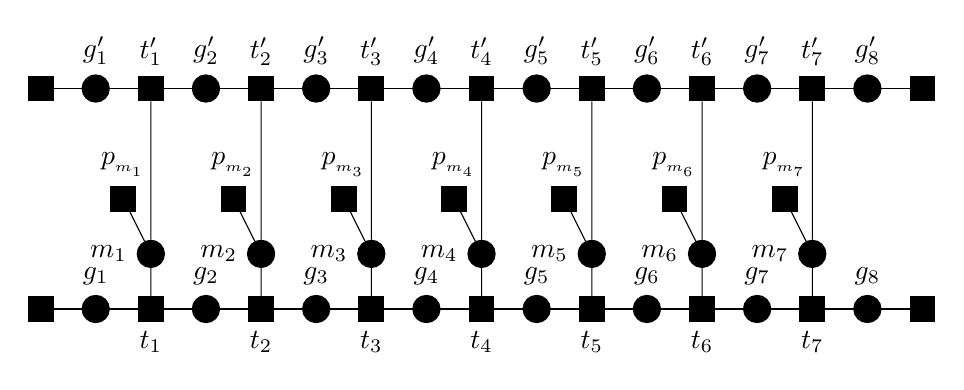
\begin{tikzpicture}[scale=0.35]
\tikzstyle{factor}=[rectangle,minimum size = 3mm, thick, draw =black,fill=black]
\tikzstyle{var}=[circle,minimum size = 3mm, thick, draw =black,fill=black]
\tikzstyle{second}=[circle, minimum size = 5mm, thick]
\tikzstyle{box}=[rectangle, draw=black!100]
\tikzstyle{connect}=[-latex, thick]

	   \pgfmathsetmacro{\posh}{-1};	
	   
	\node[factor] (tphi0) at (0,0) [label=below:{}]{};
	\node[var] (phi0) at (2,0) [label=above:{$\st{1}$}]{};
	\node[factor] (tphi1) at (4,0) [label=below:{$t_1$}]{};
	\node[var] (s0) at (4,2) [label=left:{$\x_1$}]{};
	\node[factor] (fs0) at (\posh+4,4) [label=above:{$\p{m_1}$}]{};
	
	\node[var] (phi1) at (6,0) [label=above:{$\st{2}$}]{};
	\node[factor] (tphi2) at (8,0) [label=below:{$t_2$}]{};
	\node[var] (s1) at (8,2) [label=left:{$\x_2$}]{};
	\node[factor] (fs1) at (\posh+8,4) [label=above:{$\p{\x_2}$}]{};	

	
	\node[var] (phi2) at (10,0) [label=above:{$\st{3}$}]{};
	\node[factor] (tphi3) at (12,0) [label=below:{$t_3$}]{};
		\node[var] (s2) at (12,2) [label=left:{$\x_3$}]{};
	\node[factor] (fs2) at (\posh+12,4) [label=above:{$\p{\x_3}$}]{};		
	
	\node[var] (phi3) at (14,0) [label=above:{$\st{4}$}]{};
	\node[factor] (tphi4) at (16,0) [label=below:{$t_4$}]{};
	\node[var] (s3) at (16,2) [label=left:{$\x_4$}]{};	
	\node[factor] (fs3) at (\posh+16,4) [label=above:{$\p{\x_4}$}]{};
	
	\node[var] (phi4) at (18,0) [label=above:{$\st{5}$}]{};
	\node[factor] (tphi5) at (20,0) [label=below:{$t_5$}]{};
	\node[var] (s4) at (20,2) [label=left:{$\x_5$}]{};	
	\node[factor] (fs4) at (\posh+20,4) [label=above:{$\p{\x_5}$}]{};	
	
	\node[factor] (fs5) at (\posh+24,4) [label=above:{$\p{\x_6}$}]{};	
	\node[var] (s5) at (24,2) [label=left:{$\x_6$}]{};	
	\node[var] (phi5) at (22,0) [label=above:{$\st{6}$}]{};
	\node[factor] (tphi6) at (24,0) [label=below:{$t_6$}]{};	
	
	\node[factor] (fs6) at (\posh+28,4) [label=above:{$\p{\x_7}$}]{};	
	\node[var] (s6) at (28,2) [label=left:{$\x_7$}]{};	
	\node[var] (phi6) at (26,0) [label=above:{$\st{7}$}]{};
	\node[factor] (tphi7) at (28,0) [label=below:{$t_7$}]{};
	\node[var] (phi7) at (30,0) [label=above:{$\st{8}$}]{};
	\node[factor] (tphi8) at (32,0) [label=below:{}]{};
	
	\path
		(tphi0) edge [] (tphi8)
		(fs0) edge [] (s0)
		(s0) edge [] (tphi1)
		(fs1) edge [] (s1)
		(s1) edge [] (tphi2)
		(fs2) edge [] (s2)
		(s2) edge [] (tphi3)
		(fs3) edge [] (s3)
		(s3) edge [] (tphi4)		
		(fs4) edge [] (s4)
		(s4) edge [] (tphi5)
		(fs5) edge [] (s5)
		(s5) edge [] (tphi6)	
		(fs6) edge [] (s6)
		(s6) edge [] (tphi7);	
		
		
   
   \pgfmathsetmacro{\posv}{+8};
   \pgfmathsetmacro{\posh}{0};				
		
		
	\node[factor] (tphi02) at (0,\posv+0) [label=above:{}]{};
	\node[var] (phi02) at (2,\posv+0) [label=above:{$\stp{1}$}]{};
	\node[factor] (tphi12) at (4,\posv+0) [label=above:{$t'_1$}]{};
	
	\node[var] (phi12) at (6,\posv+0) [label=above:{$\stp{2}$}]{};
	\node[factor] (tphi22) at (8,\posv+0) [label=above:{$t'_2$}]{};
	

	
	\node[var] (phi22) at (10,\posv+0) [label=above:{$\stp{3}$}]{};
	\node[factor] (tphi32) at (12,\posv+0) [label=above:{$t'_3$}]{};
	
	
	\node[var] (phi32) at (14,\posv+0) [label=above:{$\stp{4}$}]{};
	\node[factor] (tphi42) at (16,\posv+0) [label=above:{$t'_4$}]{};

	
	\node[var] (phi42) at (18,\posv+0) [label=above:{$\stp{5}$}]{};
	\node[factor] (tphi52) at (20,\posv+0) [label=above:{$t'_5$}]{};

	\node[var] (phi52) at (22,\posv+0) [label=above:{$\stp{6}$}]{};
	\node[factor] (tphi62) at (24,\posv+0) [label=above:{$t'_6$}]{};	
	
	\node[var] (phi62) at (26,\posv+0) [label=above:{$\stp{7}$}]{};
	\node[factor] (tphi72) at (28,\posv+0) [label=above:{$t'_7$}]{};
	\node[var] (phi72) at (30,\posv+0) [label=above:{$\stp{8}$}]{};
	\node[factor] (tphi82) at (32,\posv+0) [label=above:{}]{};
	
	
	\path (tphi02) edge [] (tphi82)
		    (s0) edge [] (tphi12)
	            (s1) edge [] (tphi22)
	            (s2) edge [] (tphi32)
	            (s3) edge [] (tphi42)
	            (s4) edge [] (tphi52)
	            (s5) edge [] (tphi62)
	            (s6) edge [] (tphi72);

\end{tikzpicture}
   
 
\end{center}
\end{figure}


}

\frame{
\frametitle{$\p{\mathbf{X}|\mathbf{y}}(\x)$ factor graph}



\begin{figure}[h!]
\begin{center}
\tikzset{external/remake next}
\input{tikzfiles/Fig4.tex} 
\end{center}
\end{figure}

\noteG{The FG still have cycles, but they are very long if $L\rightarrow\infty$ and the interleaver is properly designed.}
}

\frame{
\frametitle{$\p{\mathbf{X}|\mathbf{y}}(\x)$ factor graph}



\begin{figure}[h!]
\begin{center}
\tikzset{external/remake next}
\input{tikzfiles/Fig4.tex} 
\end{center}
\end{figure}

\noteR{BP can be applied directly over the factor graph. However, the resulting algorithm is very complex (lots of state messages computed per iteration)}
}

\frame{
\frametitle{Sequential schedule (I)}

We consider one chain at a time. First, BP is run over the chain corresponding to code 1 and uniform priors.

\begin{figure}[h!]
\begin{center}
\tikzset{external/remake next}
\input{tikzfiles/Fig5.tex} 
\end{center}
\end{figure}


}

\frame{
\frametitle{Sequential schedule (II)}

Then, BP is run over the second chain using the priors estimated in the previous step.

\begin{figure}[h!]
\begin{center}
\tikzset{external/remake next}
% This file was created by matlab2tikz.
% Minimal pgfplots version: 1.3
%
%The latest updates can be retrieved from
%  http://www.mathworks.com/matlabcentral/fileexchange/22022-matlab2tikz
%where you can also make suggestions and rate matlab2tikz.
%


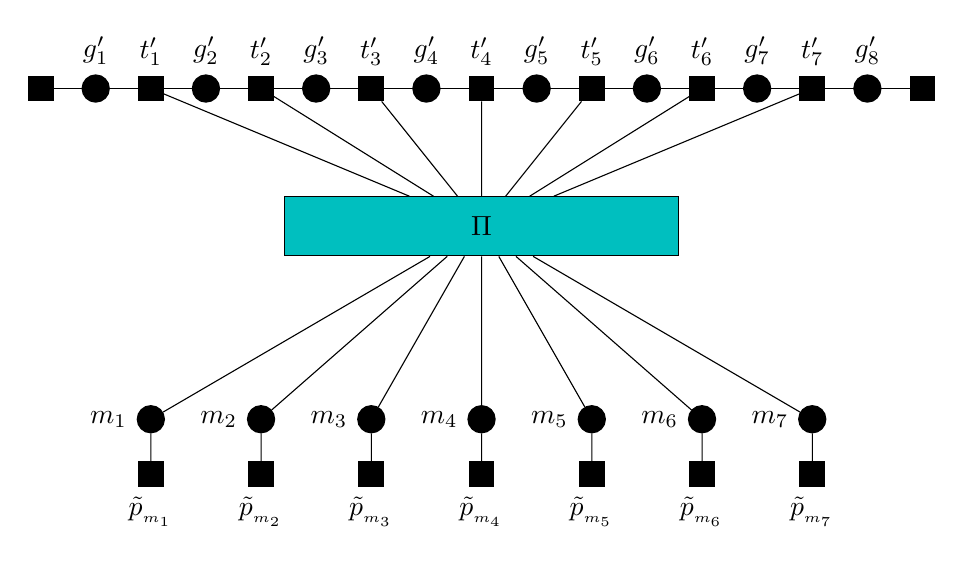
\begin{tikzpicture}[scale=0.35,
        block4/.style  = {draw, rectangle, minimum width = 5cm, minimum height = 0.75cm,fill=mycolor2},
]
\tikzstyle{factor}=[rectangle,minimum size = 3mm, thick, draw =black,fill=black]
\tikzstyle{var}=[circle,minimum size = 3mm, thick, draw =black,fill=black]
\tikzstyle{second}=[circle, minimum size = 5mm, thick]
\tikzstyle{box}=[rectangle, draw=black!100]
\tikzstyle{connect}=[-latex, thick]


	   \pgfmathsetmacro{\posh}{0};	
	     

	\node[var] (s0) at (4,2) [label=left:{$\x_1$}]{};
	\node[factor] (fs0) at (\posh+4,0) [label=below:{$\pmd{\x_1}$}]{};

	\node[var] (s1) at (8,2) [label=left:{$\x_2$}]{};
	\node[factor] (fs1) at (\posh+8,0) [label=below:{$\pmd{\x_2}$}]{};	

		\node[var] (s2) at (12,2) [label=left:{$\x_3$}]{};
	\node[factor] (fs2) at (\posh+12,0) [label=below:{$\pmd{\x_3}$}]{};		

	\node[var] (s3) at (16,2) [label=left:{$\x_4$}]{};	
	\node[factor] (fs3) at (\posh+16,0) [label=below:{$\pmd{\x_4}$}]{};
	

	\node[var] (s4) at (20,2) [label=left:{$\x_5$}]{};	
	\node[factor] (fs4) at (\posh+20,0) [label=below:{$\pmd{\x_5}$}]{};	
	
	\node[factor] (fs5) at (\posh+24,0) [label=below:{$\pmd{\x_6}$}]{};	
	\node[var] (s5) at (24,2) [label=left:{$\x_6$}]{};	

	
	\node[factor] (fs6) at (\posh+28,0) [label=below:{$\pmd{\x_7}$}]{};	
	\node[var] (s6) at (28,2) [label=left:{$\x_7$}]{};	
	
	\path
		(fs0) edge [] (s0)
		(fs1) edge [] (s1)
		(fs2) edge [] (s2)
		(fs3) edge [] (s3)	
		(fs4) edge [] (s4)
		(fs5) edge [] (s5)
		(fs6) edge [] (s6);	
		
		
   
   \pgfmathsetmacro{\posv}{+9};
   
     \draw (16,\posv) node[block4]  (Int) {$\Pi$};  
     
     \pgfmathsetmacro{\posv}{14};
     
   \pgfmathsetmacro{\posh}{0};				
		
		
	\node[factor] (tphi02) at (0,\posv+0) [label=above:{}]{};
	\node[var] (phi02) at (2,\posv+0) [label=above:{$\stp{1}$}]{};
	\node[factor] (tphi12) at (4,\posv+0) [label=above:{$t'_1$}]{};
	
	\node[var] (phi12) at (6,\posv+0) [label=above:{$\stp{2}$}]{};
	\node[factor] (tphi22) at (8,\posv+0) [label=above:{$t'_2$}]{};
	

	
	\node[var] (phi22) at (10,\posv+0) [label=above:{$\stp{3}$}]{};
	\node[factor] (tphi32) at (12,\posv+0) [label=above:{$t'_3$}]{};
	
	
	\node[var] (phi32) at (14,\posv+0) [label=above:{$\stp{4}$}]{};
	\node[factor] (tphi42) at (16,\posv+0) [label=above:{$t'_4$}]{};

	
	\node[var] (phi42) at (18,\posv+0) [label=above:{$\stp{5}$}]{};
	\node[factor] (tphi52) at (20,\posv+0) [label=above:{$t'_5$}]{};

	\node[var] (phi52) at (22,\posv+0) [label=above:{$\stp{6}$}]{};
	\node[factor] (tphi62) at (24,\posv+0) [label=above:{$t'_6$}]{};	
	
	\node[var] (phi62) at (26,\posv+0) [label=above:{$\stp{7}$}]{};
	\node[factor] (tphi72) at (28,\posv+0) [label=above:{$t'_7$}]{};
	\node[var] (phi72) at (30,\posv+0) [label=above:{$\stp{8}$}]{};
	\node[factor] (tphi82) at (32,\posv+0) [label=above:{}]{};
	
	
	\path (tphi02) edge [] (tphi82)
		    (Int) edge [] (tphi12)
	            (Int)edge [] (tphi22)
	            (Int) edge [] (tphi32)
	            (Int) edge [] (tphi42)
	            (Int) edge [] (tphi52)
	            (Int) edge [] (tphi62)
	            (Int) edge [] (tphi72)
	             (s0) edge [] (Int)
	            (s1) edge [] (Int)
	            (s2) edge [] (Int)
	            (s3) edge [] (Int)
	            (s4) edge [] (Int)
	            (s5) edge [] (Int)
	            (s6) edge [] (Int);

\end{tikzpicture}
   
 
\end{center}
\end{figure}


}

\frame{
\frametitle{Sequential schedule (III)}

BP is run over the first chain using the priors estimated in the previous step.

\begin{figure}[h!]
\begin{center}
\tikzset{external/remake next}
% This file was created by matlab2tikz.
% Minimal pgfplots version: 1.3
%
%The latest updates can be retrieved from
%  http://www.mathworks.com/matlabcentral/fileexchange/22022-matlab2tikz
%where you can also make suggestions and rate matlab2tikz.
%


\begin{tikzpicture}[scale=0.35,
        block4/.style  = {draw=mycolor3, rectangle, minimum width = 5cm, minimum height = 0.75cm,fill=mycolor3},
]
\tikzstyle{factor}=[rectangle,minimum size = 3mm, thick, draw =black,fill=black]
\tikzstyle{var}=[circle,minimum size = 3mm, thick, draw =black,fill=black]
\tikzstyle{second}=[circle, minimum size = 5mm, thick]
\tikzstyle{box}=[rectangle, draw=black!100]
\tikzstyle{connect}=[-latex, thick]


	   \pgfmathsetmacro{\posh}{-1};	
	   
	\node[factor] (tphi0) at (0,0) [label=below:{}]{};
	\node[var] (phi0) at (2,0) [label=above:{$\st{1}$}]{};
	\node[factor] (tphi1) at (4,0) [label=below:{$t_1$}]{};
	\node[var] (s0) at (4,2) [label=left:{$\x_1$}]{};
	\node[factor] (fs0) at (\posh+4,4) [label=above:{$\pmd{\x_1}$}]{};
	
	\node[var] (phi1) at (6,0) [label=above:{$\st{2}$}]{};
	\node[factor] (tphi2) at (8,0) [label=below:{$t_2$}]{};
	\node[var] (s1) at (8,2) [label=left:{$\x_2$}]{};
	\node[factor] (fs1) at (\posh+8,4) [label=above:{$\pmd{\x_2}$}]{};	

	
	\node[var] (phi2) at (10,0) [label=above:{$\st{3}$}]{};
	\node[factor] (tphi3) at (12,0) [label=below:{$t_3$}]{};
		\node[var] (s2) at (12,2) [label=left:{$\x_3$}]{};
	\node[factor] (fs2) at (\posh+12,4) [label=above:{$\pmd{\x_3}$}]{};		
	
	\node[var] (phi3) at (14,0) [label=above:{$\st{4}$}]{};
	\node[factor] (tphi4) at (16,0) [label=below:{$t_4$}]{};
	\node[var] (s3) at (16,2) [label=left:{$\x_4$}]{};	
	\node[factor] (fs3) at (\posh+16,4) [label=above:{$\pmd{\x_4}$}]{};
	
	\node[var] (phi4) at (18,0) [label=above:{$\st{5}$}]{};
	\node[factor] (tphi5) at (20,0) [label=below:{$t_5$}]{};
	\node[var] (s4) at (20,2) [label=left:{$\x_5$}]{};	
	\node[factor] (fs4) at (\posh+20,4) [label=above:{$\pmd{\x_5}$}]{};	
	
	\node[factor] (fs5) at (\posh+24,4) [label=above:{$\pmd{\x_6}$}]{};	
	\node[var] (s5) at (24,2) [label=left:{$\x_6$}]{};	
	\node[var] (phi5) at (22,0) [label=above:{$\st{6}$}]{};
	\node[factor] (tphi6) at (24,0) [label=below:{$t_6$}]{};	
	
	\node[factor] (fs6) at (\posh+28,4) [label=above:{$\pmd{\x_7}$}]{};	
	\node[var] (s6) at (28,2) [label=left:{$\x_7$}]{};	
	\node[var] (phi6) at (26,0) [label=above:{$\st{7}$}]{};
	\node[factor] (tphi7) at (28,0) [label=below:{$t_7$}]{};
	\node[var] (phi7) at (30,0) [label=above:{$\st{8}$}]{};
	\node[factor] (tphi8) at (32,0) [label=below:{}]{};
	
	\path
		(tphi0) edge [] (tphi8)
		(fs0) edge [] (s0)
		(s0) edge [] (tphi1)
		(fs1) edge [] (s1)
		(s1) edge [] (tphi2)
		(fs2) edge [] (s2)
		(s2) edge [] (tphi3)
		(fs3) edge [] (s3)
		(s3) edge [] (tphi4)		
		(fs4) edge [] (s4)
		(s4) edge [] (tphi5)
		(fs5) edge [] (s5)
		(s5) edge [] (tphi6)	
		(fs6) edge [] (s6)
		(s6) edge [] (tphi7);	
%\begin{figure}[h!]
%\begin{center}
%\tikzset{external/remake next}
%% This file was created by matlab2tikz.
% Minimal pgfplots version: 1.3
%
%The latest updates can be retrieved from
%  http://www.mathworks.com/matlabcentral/fileexchange/22022-matlab2tikz
%where you can also make suggestions and rate matlab2tikz.
%


\begin{tikzpicture}[scale=0.35,
        block4/.style  = {draw=mycolor3, rectangle, minimum width = 5cm, minimum height = 0.75cm,fill=mycolor3},
]
\tikzstyle{factor}=[rectangle,minimum size = 3mm, thick, draw =black,fill=black]
\tikzstyle{var}=[circle,minimum size = 3mm, thick, draw =black,fill=black]
\tikzstyle{second}=[circle, minimum size = 5mm, thick]
\tikzstyle{box}=[rectangle, draw=black!100]
\tikzstyle{connect}=[-latex, thick]


	   \pgfmathsetmacro{\posh}{-1};	
	   
	\node[factor] (tphi0) at (0,0) [label=below:{}]{};
	\node[var] (phi0) at (2,0) [label=above:{$\st{1}$}]{};
	\node[factor] (tphi1) at (4,0) [label=below:{$t_1$}]{};
	\node[var] (s0) at (4,2) [label=left:{$\x_1$}]{};
	\node[factor] (fs0) at (\posh+4,4) [label=above:{$\pmd{\x_1}$}]{};
	
	\node[var] (phi1) at (6,0) [label=above:{$\st{2}$}]{};
	\node[factor] (tphi2) at (8,0) [label=below:{$t_2$}]{};
	\node[var] (s1) at (8,2) [label=left:{$\x_2$}]{};
	\node[factor] (fs1) at (\posh+8,4) [label=above:{$\pmd{\x_2}$}]{};	

	
	\node[var] (phi2) at (10,0) [label=above:{$\st{3}$}]{};
	\node[factor] (tphi3) at (12,0) [label=below:{$t_3$}]{};
		\node[var] (s2) at (12,2) [label=left:{$\x_3$}]{};
	\node[factor] (fs2) at (\posh+12,4) [label=above:{$\pmd{\x_3}$}]{};		
	
	\node[var] (phi3) at (14,0) [label=above:{$\st{4}$}]{};
	\node[factor] (tphi4) at (16,0) [label=below:{$t_4$}]{};
	\node[var] (s3) at (16,2) [label=left:{$\x_4$}]{};	
	\node[factor] (fs3) at (\posh+16,4) [label=above:{$\pmd{\x_4}$}]{};
	
	\node[var] (phi4) at (18,0) [label=above:{$\st{5}$}]{};
	\node[factor] (tphi5) at (20,0) [label=below:{$t_5$}]{};
	\node[var] (s4) at (20,2) [label=left:{$\x_5$}]{};	
	\node[factor] (fs4) at (\posh+20,4) [label=above:{$\pmd{\x_5}$}]{};	
	
	\node[factor] (fs5) at (\posh+24,4) [label=above:{$\pmd{\x_6}$}]{};	
	\node[var] (s5) at (24,2) [label=left:{$\x_6$}]{};	
	\node[var] (phi5) at (22,0) [label=above:{$\st{6}$}]{};
	\node[factor] (tphi6) at (24,0) [label=below:{$t_6$}]{};	
	
	\node[factor] (fs6) at (\posh+28,4) [label=above:{$\pmd{\x_7}$}]{};	
	\node[var] (s6) at (28,2) [label=left:{$\x_7$}]{};	
	\node[var] (phi6) at (26,0) [label=above:{$\st{7}$}]{};
	\node[factor] (tphi7) at (28,0) [label=below:{$t_7$}]{};
	\node[var] (phi7) at (30,0) [label=above:{$\st{8}$}]{};
	\node[factor] (tphi8) at (32,0) [label=below:{}]{};
	
	\path
		(tphi0) edge [] (tphi8)
		(fs0) edge [] (s0)
		(s0) edge [] (tphi1)
		(fs1) edge [] (s1)
		(s1) edge [] (tphi2)
		(fs2) edge [] (s2)
		(s2) edge [] (tphi3)
		(fs3) edge [] (s3)
		(s3) edge [] (tphi4)		
		(fs4) edge [] (s4)
		(s4) edge [] (tphi5)
		(fs5) edge [] (s5)
		(s5) edge [] (tphi6)	
		(fs6) edge [] (s6)
		(s6) edge [] (tphi7);	
%\begin{figure}[h!]
%\begin{center}
%\tikzset{external/remake next}
%% This file was created by matlab2tikz.
% Minimal pgfplots version: 1.3
%
%The latest updates can be retrieved from
%  http://www.mathworks.com/matlabcentral/fileexchange/22022-matlab2tikz
%where you can also make suggestions and rate matlab2tikz.
%


\begin{tikzpicture}[scale=0.35,
        block4/.style  = {draw=mycolor3, rectangle, minimum width = 5cm, minimum height = 0.75cm,fill=mycolor3},
]
\tikzstyle{factor}=[rectangle,minimum size = 3mm, thick, draw =black,fill=black]
\tikzstyle{var}=[circle,minimum size = 3mm, thick, draw =black,fill=black]
\tikzstyle{second}=[circle, minimum size = 5mm, thick]
\tikzstyle{box}=[rectangle, draw=black!100]
\tikzstyle{connect}=[-latex, thick]


	   \pgfmathsetmacro{\posh}{-1};	
	   
	\node[factor] (tphi0) at (0,0) [label=below:{}]{};
	\node[var] (phi0) at (2,0) [label=above:{$\st{1}$}]{};
	\node[factor] (tphi1) at (4,0) [label=below:{$t_1$}]{};
	\node[var] (s0) at (4,2) [label=left:{$\x_1$}]{};
	\node[factor] (fs0) at (\posh+4,4) [label=above:{$\pmd{\x_1}$}]{};
	
	\node[var] (phi1) at (6,0) [label=above:{$\st{2}$}]{};
	\node[factor] (tphi2) at (8,0) [label=below:{$t_2$}]{};
	\node[var] (s1) at (8,2) [label=left:{$\x_2$}]{};
	\node[factor] (fs1) at (\posh+8,4) [label=above:{$\pmd{\x_2}$}]{};	

	
	\node[var] (phi2) at (10,0) [label=above:{$\st{3}$}]{};
	\node[factor] (tphi3) at (12,0) [label=below:{$t_3$}]{};
		\node[var] (s2) at (12,2) [label=left:{$\x_3$}]{};
	\node[factor] (fs2) at (\posh+12,4) [label=above:{$\pmd{\x_3}$}]{};		
	
	\node[var] (phi3) at (14,0) [label=above:{$\st{4}$}]{};
	\node[factor] (tphi4) at (16,0) [label=below:{$t_4$}]{};
	\node[var] (s3) at (16,2) [label=left:{$\x_4$}]{};	
	\node[factor] (fs3) at (\posh+16,4) [label=above:{$\pmd{\x_4}$}]{};
	
	\node[var] (phi4) at (18,0) [label=above:{$\st{5}$}]{};
	\node[factor] (tphi5) at (20,0) [label=below:{$t_5$}]{};
	\node[var] (s4) at (20,2) [label=left:{$\x_5$}]{};	
	\node[factor] (fs4) at (\posh+20,4) [label=above:{$\pmd{\x_5}$}]{};	
	
	\node[factor] (fs5) at (\posh+24,4) [label=above:{$\pmd{\x_6}$}]{};	
	\node[var] (s5) at (24,2) [label=left:{$\x_6$}]{};	
	\node[var] (phi5) at (22,0) [label=above:{$\st{6}$}]{};
	\node[factor] (tphi6) at (24,0) [label=below:{$t_6$}]{};	
	
	\node[factor] (fs6) at (\posh+28,4) [label=above:{$\pmd{\x_7}$}]{};	
	\node[var] (s6) at (28,2) [label=left:{$\x_7$}]{};	
	\node[var] (phi6) at (26,0) [label=above:{$\st{7}$}]{};
	\node[factor] (tphi7) at (28,0) [label=below:{$t_7$}]{};
	\node[var] (phi7) at (30,0) [label=above:{$\st{8}$}]{};
	\node[factor] (tphi8) at (32,0) [label=below:{}]{};
	
	\path
		(tphi0) edge [] (tphi8)
		(fs0) edge [] (s0)
		(s0) edge [] (tphi1)
		(fs1) edge [] (s1)
		(s1) edge [] (tphi2)
		(fs2) edge [] (s2)
		(s2) edge [] (tphi3)
		(fs3) edge [] (s3)
		(s3) edge [] (tphi4)		
		(fs4) edge [] (s4)
		(s4) edge [] (tphi5)
		(fs5) edge [] (s5)
		(s5) edge [] (tphi6)	
		(fs6) edge [] (s6)
		(s6) edge [] (tphi7);	
%\begin{figure}[h!]
%\begin{center}
%\tikzset{external/remake next}
%\input{tikzfiles/Fig7.tex} 
%\end{center}
%\end{figure}

		
		
   
   \pgfmathsetmacro{\posv}{+9};
   
     \draw (16,\posv) node[block4]  (Int) {$\Pi$};  
     
     \pgfmathsetmacro{\posv}{14};
     
   \pgfmathsetmacro{\posh}{0};			
   
   
   \tikzstyle{factor}=[rectangle,minimum size = 3mm,  draw =mycolor3,fill=mycolor3]
\tikzstyle{var}=[circle,minimum size = 3mm, draw =mycolor3,fill=mycolor3]
\tikzstyle{second}=[circle, minimum size = 5mm, thick]
\tikzstyle{box}=[rectangle, draw=black!100]
\tikzstyle{connect}=[-latex, thick]	
		
		
	\node[factor] (tphi02) at (0,\posv+0) [label=above:{}]{};
	\node[var] (phi02) at (2,\posv+0) [label=above:{$\stp{1}$}]{};
	\node[factor] (tphi12) at (4,\posv+0) [label=above:{$t'_1$}]{};
	
	\node[var] (phi12) at (6,\posv+0) [label=above:{$\stp{2}$}]{};
	\node[factor] (tphi22) at (8,\posv+0) [label=above:{$t'_2$}]{};
	

	
	\node[var] (phi22) at (10,\posv+0) [label=above:{$\stp{3}$}]{};
	\node[factor] (tphi32) at (12,\posv+0) [label=above:{$t'_3$}]{};
	
	
	\node[var] (phi32) at (14,\posv+0) [label=above:{$\stp{4}$}]{};
	\node[factor] (tphi42) at (16,\posv+0) [label=above:{$t'_4$}]{};

	
	\node[var] (phi42) at (18,\posv+0) [label=above:{$\stp{5}$}]{};
	\node[factor] (tphi52) at (20,\posv+0) [label=above:{$t'_5$}]{};

	\node[var] (phi52) at (22,\posv+0) [label=above:{$\stp{6}$}]{};
	\node[factor] (tphi62) at (24,\posv+0) [label=above:{$t'_6$}]{};	
	
	\node[var] (phi62) at (26,\posv+0) [label=above:{$\stp{7}$}]{};
	\node[factor] (tphi72) at (28,\posv+0) [label=above:{$t'_7$}]{};
	\node[var] (phi72) at (30,\posv+0) [label=above:{$\stp{8}$}]{};
	\node[factor] (tphi82) at (32,\posv+0) [label=above:{}]{};
	
	
	\path[mycolor3] (tphi02) edge [] (tphi82)
		    (Int) edge [] (tphi12)
	            (Int)edge [] (tphi22)
	            (Int) edge [] (tphi32)
	            (Int) edge [] (tphi42)
	            (Int) edge [] (tphi52)
	            (Int) edge [] (tphi62)
	            (Int) edge [] (tphi72)
	             (s0) edge [] (Int)
	            (s1) edge [] (Int)
	            (s2) edge [] (Int)
	            (s3) edge [] (Int)
	            (s4) edge [] (Int)
	            (s5) edge [] (Int)
	            (s6) edge [] (Int);

\end{tikzpicture}
   
 
%\end{center}
%\end{figure}

		
		
   
   \pgfmathsetmacro{\posv}{+9};
   
     \draw (16,\posv) node[block4]  (Int) {$\Pi$};  
     
     \pgfmathsetmacro{\posv}{14};
     
   \pgfmathsetmacro{\posh}{0};			
   
   
   \tikzstyle{factor}=[rectangle,minimum size = 3mm,  draw =mycolor3,fill=mycolor3]
\tikzstyle{var}=[circle,minimum size = 3mm, draw =mycolor3,fill=mycolor3]
\tikzstyle{second}=[circle, minimum size = 5mm, thick]
\tikzstyle{box}=[rectangle, draw=black!100]
\tikzstyle{connect}=[-latex, thick]	
		
		
	\node[factor] (tphi02) at (0,\posv+0) [label=above:{}]{};
	\node[var] (phi02) at (2,\posv+0) [label=above:{$\stp{1}$}]{};
	\node[factor] (tphi12) at (4,\posv+0) [label=above:{$t'_1$}]{};
	
	\node[var] (phi12) at (6,\posv+0) [label=above:{$\stp{2}$}]{};
	\node[factor] (tphi22) at (8,\posv+0) [label=above:{$t'_2$}]{};
	

	
	\node[var] (phi22) at (10,\posv+0) [label=above:{$\stp{3}$}]{};
	\node[factor] (tphi32) at (12,\posv+0) [label=above:{$t'_3$}]{};
	
	
	\node[var] (phi32) at (14,\posv+0) [label=above:{$\stp{4}$}]{};
	\node[factor] (tphi42) at (16,\posv+0) [label=above:{$t'_4$}]{};

	
	\node[var] (phi42) at (18,\posv+0) [label=above:{$\stp{5}$}]{};
	\node[factor] (tphi52) at (20,\posv+0) [label=above:{$t'_5$}]{};

	\node[var] (phi52) at (22,\posv+0) [label=above:{$\stp{6}$}]{};
	\node[factor] (tphi62) at (24,\posv+0) [label=above:{$t'_6$}]{};	
	
	\node[var] (phi62) at (26,\posv+0) [label=above:{$\stp{7}$}]{};
	\node[factor] (tphi72) at (28,\posv+0) [label=above:{$t'_7$}]{};
	\node[var] (phi72) at (30,\posv+0) [label=above:{$\stp{8}$}]{};
	\node[factor] (tphi82) at (32,\posv+0) [label=above:{}]{};
	
	
	\path[mycolor3] (tphi02) edge [] (tphi82)
		    (Int) edge [] (tphi12)
	            (Int)edge [] (tphi22)
	            (Int) edge [] (tphi32)
	            (Int) edge [] (tphi42)
	            (Int) edge [] (tphi52)
	            (Int) edge [] (tphi62)
	            (Int) edge [] (tphi72)
	             (s0) edge [] (Int)
	            (s1) edge [] (Int)
	            (s2) edge [] (Int)
	            (s3) edge [] (Int)
	            (s4) edge [] (Int)
	            (s5) edge [] (Int)
	            (s6) edge [] (Int);

\end{tikzpicture}
   
 
%\end{center}
%\end{figure}

		
		
   
   \pgfmathsetmacro{\posv}{+9};
   
     \draw (16,\posv) node[block4]  (Int) {$\Pi$};  
     
     \pgfmathsetmacro{\posv}{14};
     
   \pgfmathsetmacro{\posh}{0};			
   
   
   \tikzstyle{factor}=[rectangle,minimum size = 3mm,  draw =mycolor3,fill=mycolor3]
\tikzstyle{var}=[circle,minimum size = 3mm, draw =mycolor3,fill=mycolor3]
\tikzstyle{second}=[circle, minimum size = 5mm, thick]
\tikzstyle{box}=[rectangle, draw=black!100]
\tikzstyle{connect}=[-latex, thick]	
		
		
	\node[factor] (tphi02) at (0,\posv+0) [label=above:{}]{};
	\node[var] (phi02) at (2,\posv+0) [label=above:{$\stp{1}$}]{};
	\node[factor] (tphi12) at (4,\posv+0) [label=above:{$t'_1$}]{};
	
	\node[var] (phi12) at (6,\posv+0) [label=above:{$\stp{2}$}]{};
	\node[factor] (tphi22) at (8,\posv+0) [label=above:{$t'_2$}]{};
	

	
	\node[var] (phi22) at (10,\posv+0) [label=above:{$\stp{3}$}]{};
	\node[factor] (tphi32) at (12,\posv+0) [label=above:{$t'_3$}]{};
	
	
	\node[var] (phi32) at (14,\posv+0) [label=above:{$\stp{4}$}]{};
	\node[factor] (tphi42) at (16,\posv+0) [label=above:{$t'_4$}]{};

	
	\node[var] (phi42) at (18,\posv+0) [label=above:{$\stp{5}$}]{};
	\node[factor] (tphi52) at (20,\posv+0) [label=above:{$t'_5$}]{};

	\node[var] (phi52) at (22,\posv+0) [label=above:{$\stp{6}$}]{};
	\node[factor] (tphi62) at (24,\posv+0) [label=above:{$t'_6$}]{};	
	
	\node[var] (phi62) at (26,\posv+0) [label=above:{$\stp{7}$}]{};
	\node[factor] (tphi72) at (28,\posv+0) [label=above:{$t'_7$}]{};
	\node[var] (phi72) at (30,\posv+0) [label=above:{$\stp{8}$}]{};
	\node[factor] (tphi82) at (32,\posv+0) [label=above:{}]{};
	
	
	\path[mycolor3] (tphi02) edge [] (tphi82)
		    (Int) edge [] (tphi12)
	            (Int)edge [] (tphi22)
	            (Int) edge [] (tphi32)
	            (Int) edge [] (tphi42)
	            (Int) edge [] (tphi52)
	            (Int) edge [] (tphi62)
	            (Int) edge [] (tphi72)
	             (s0) edge [] (Int)
	            (s1) edge [] (Int)
	            (s2) edge [] (Int)
	            (s3) edge [] (Int)
	            (s4) edge [] (Int)
	            (s5) edge [] (Int)
	            (s6) edge [] (Int);

\end{tikzpicture}
   
 
\end{center}
\end{figure}

\noteG{We iterate until convergence. Tipically no more than 10-15 iterations.}
}




\end{document}

